\documentclass[handout]{beamer}
%\setbeameroption{hide notes} % Only slides
%\setbeameroption{show only notes} % Only notes
\setbeameroption{show notes on second screen=right}

\usepackage{esint}
\usepackage{graphicx}
\usepackage{tikz}
\usepackage{tikz-among-us}
\usepackage{caption}
\usepackage[british]{babel}
%\usepackage{kpfonts}

% Theme (Boadilla, Hannover, metropolis, Pittsburgh)

% METROPOLIS
% Uses Fira fonts - compile with xelatex to use
% Features [standout] frames

\usetheme[progressbar=frametitle]{metropolis}

% Colours (owl, dolphin, seagull)

% OWL
% Custom colours: red, green, blue, cyan, brown, orange, yellow, violet
% Has [snowy] variant

\usecolortheme{}

\useinnertheme{}                            % Bullet point style (circles usually best)
\useoutertheme{}                       % Header/footer style
\setbeamerfont{caption}{size=\tiny}         % Caption size
\captionsetup[figure]{labelformat=empty}    % Remove figure labels
\usefonttheme[onlymath]{serif}

%\logo{\includegraphics[height=2cm]{}}
\title{Music Arrangement via Quantum Annealing}
\subtitle{}
\author{Lucas Kirby}
\institute{\color{violet} Durham University}
\date{\today}

\begin{document}

\begin{frame}
    \titlepage
\end{frame}

\begin{frame}{Overview}
    \tableofcontents
\end{frame}

\section{Theory}

\subsection{Music arrangement}

\begin{frame}{Music arrangement}
    \begin{columns}
        \begin{column}{0.6\textwidth}
            \begin{itemize}
                \item<2-> Adaptation of previously composed pieces for practical or artistic reasons
                \item<3-> Traditionally complex and time-consuming
                \item<4-> This study focuses on \textbf{reduction}
            \end{itemize}
        \end{column}
        \begin{column}{0.4\textwidth}
            \begin{figure}
                \centering
                    \includegraphics<1->[width=\textwidth]{../Figures/excerpt-1.png}
                    \caption{Beethoven's String Quartet No.\ 10}
                \end{figure}
        \end{column}
    \end{columns}
\end{frame}

\subsection{Quantum annealing}

\begin{frame}{Quantum annealing}
    \begin{itemize}
        \item<2-> \textit{Materials} | heating and cooling a material to alter its physical properties
        \item<3-> \textit{Quantum} | changing a quantum system from one Hamiltonian to another
        \item<4-> Done slowly and adiabatically to remain in the ground state
    \end{itemize}
    \vfill
    \begin{equation*}
        \onslide<5->{H(t)=\left(1- \frac{t}{T}\right)H_0 + \frac{t}{T}H_p}
    \end{equation*}
\end{frame}

\begin{frame}{QUBO}
    Encodes problem solution into Hamiltonian's ground state
    \note[item]{Lattice of spins with two discrete values}
    \note[item]{Coupling strengths $J_{ij}$ and field strengths $h_i$}
    \begin{exampleblock}{Ising model}
        \begin{equation*}
            H(s) = -\sum_{i<j}J_{ij}s_i s_j - \sum_{i=1}^{N}h_i s_i
        \end{equation*}
    \end{exampleblock}

    \note[item]{QUBO is a function to be minimised}
    \begin{alertblock}{QUBO}
        \vspace{0.1em}
        Quadratic Unconstrained Binary Optimisation
        \begin{equation*}
            f(x)=\sum_{i<j}Q_{i,j}x_ix_j + \sum_iQ_{i,i}x_i
        \end{equation*}
    \end{alertblock}
\end{frame}

\begin{frame}[standout]
    \centering
    How to combine them?
\end{frame}

\section{Methods}

\begin{frame}{Problem formulation}
    \begin{enumerate}
        \item<2-> Split parts into phrases
        \item<3-> Arrange phrases into a graph
        \item<4-> Solve graph problem using QPU
        \item<5-> Construct arrangement from solution
    \end{enumerate}
\end{frame}

\begin{frame}{1. Split parts}
    \begin{block}{}
        \centering
        Local boundary detection model (LBDM)
        \begin{equation*}
            S_i=x_i\times (r_{i-1, i} + r_{i, i+1})
        \end{equation*}
    \end{block}
    \begin{figure}
        \centering
        \includegraphics<1->[width=0.8\textwidth]{../Figures/toy-1.png}
    \end{figure}
\end{frame}

\begin{frame}{2. Create graph}
    \note{Each phrase becomes a node}
    \note{Edges between nodes if phrases overlap}

    \begin{figure}
        \centering
        \includegraphics<1->[width=0.8\textwidth]{../Figures/toy-1.png}
    \end{figure}
    \begin{figure}
        \centering
        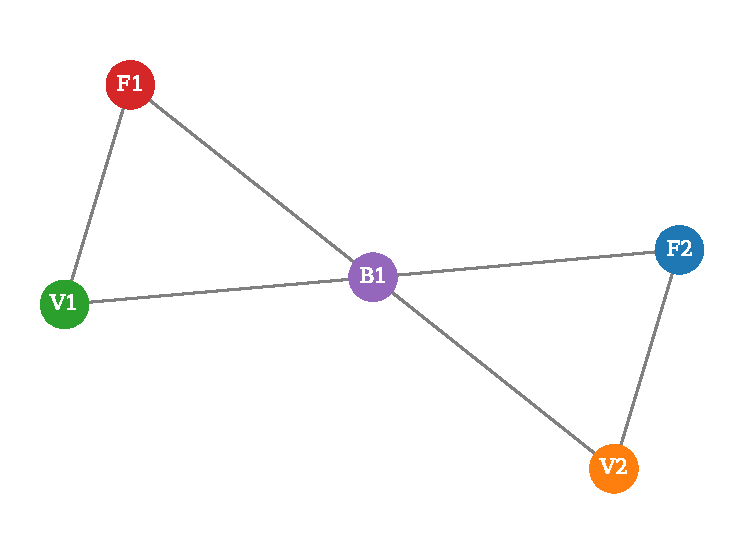
\includegraphics[width=0.5\textwidth]{../Figures/toy_graph.pdf}
    \end{figure}
\end{frame}

\begin{frame}{3. Solve graph}
    \begin{alertblock}{Maximal independent set (MIS)}
        Largest subset of nodes such that no nodes within the subset are connected by an edge.
        \begin{equation*}
            f(x)=A\sum_{ij\in E}x_ix_j-B\sum_i x_i
        \end{equation*}
    \end{alertblock}
    \begin{columns}
        \begin{column}{0.5\textwidth}
            \begin{figure}
                \centering
                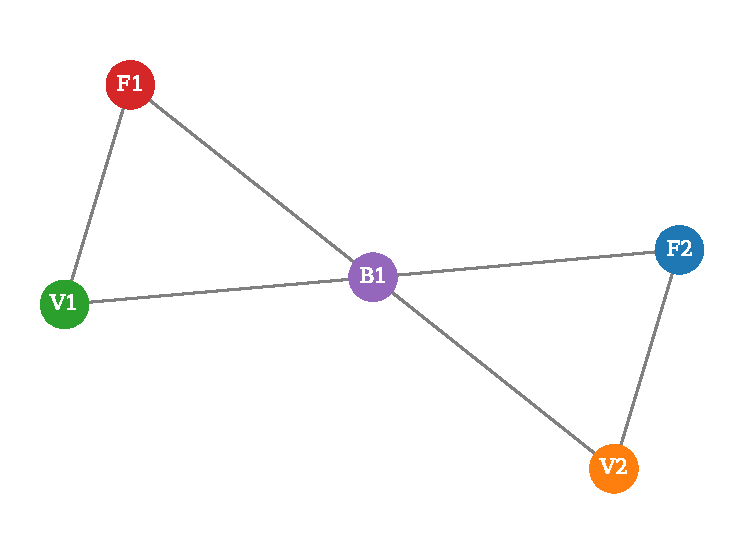
\includegraphics[width=0.9\textwidth]{../Figures/toy_graph.pdf}
            \end{figure}
        \end{column}
        \begin{column}{0.5\textwidth}
            \centering
            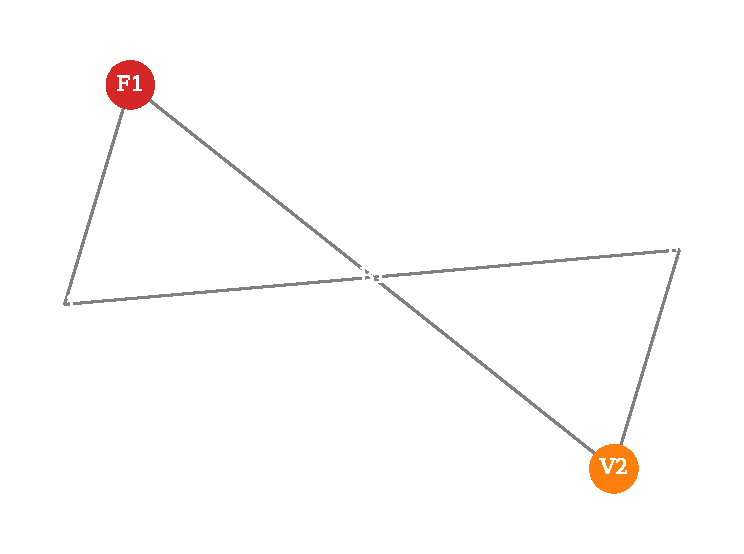
\includegraphics[width=0.9\textwidth]{../Figures/toy_solution.pdf}
        \end{column}
    \end{columns}
\end{frame}

\begin{frame}{4. Construct arrangement}
    \note{Take selected nodes and combine to create final arrangement}

    \begin{figure}
        \centering
        \includegraphics<1->[width=0.8\textwidth]{../Figures/toy-1.png}
    \end{figure}
    \centering
    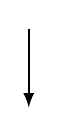
\begin{tikzpicture}
        \draw [thick, -latex](0,0) -- (0,-1);
    \end{tikzpicture}
    \begin{figure}
        \centering
        \includegraphics<2->[width=0.8\textwidth]{../Figures/toy_arrangement-1.png}
    \end{figure}
\end{frame}

\section{Results}

\begin{frame}{Excerpt}
    \begin{figure}
        \centering
        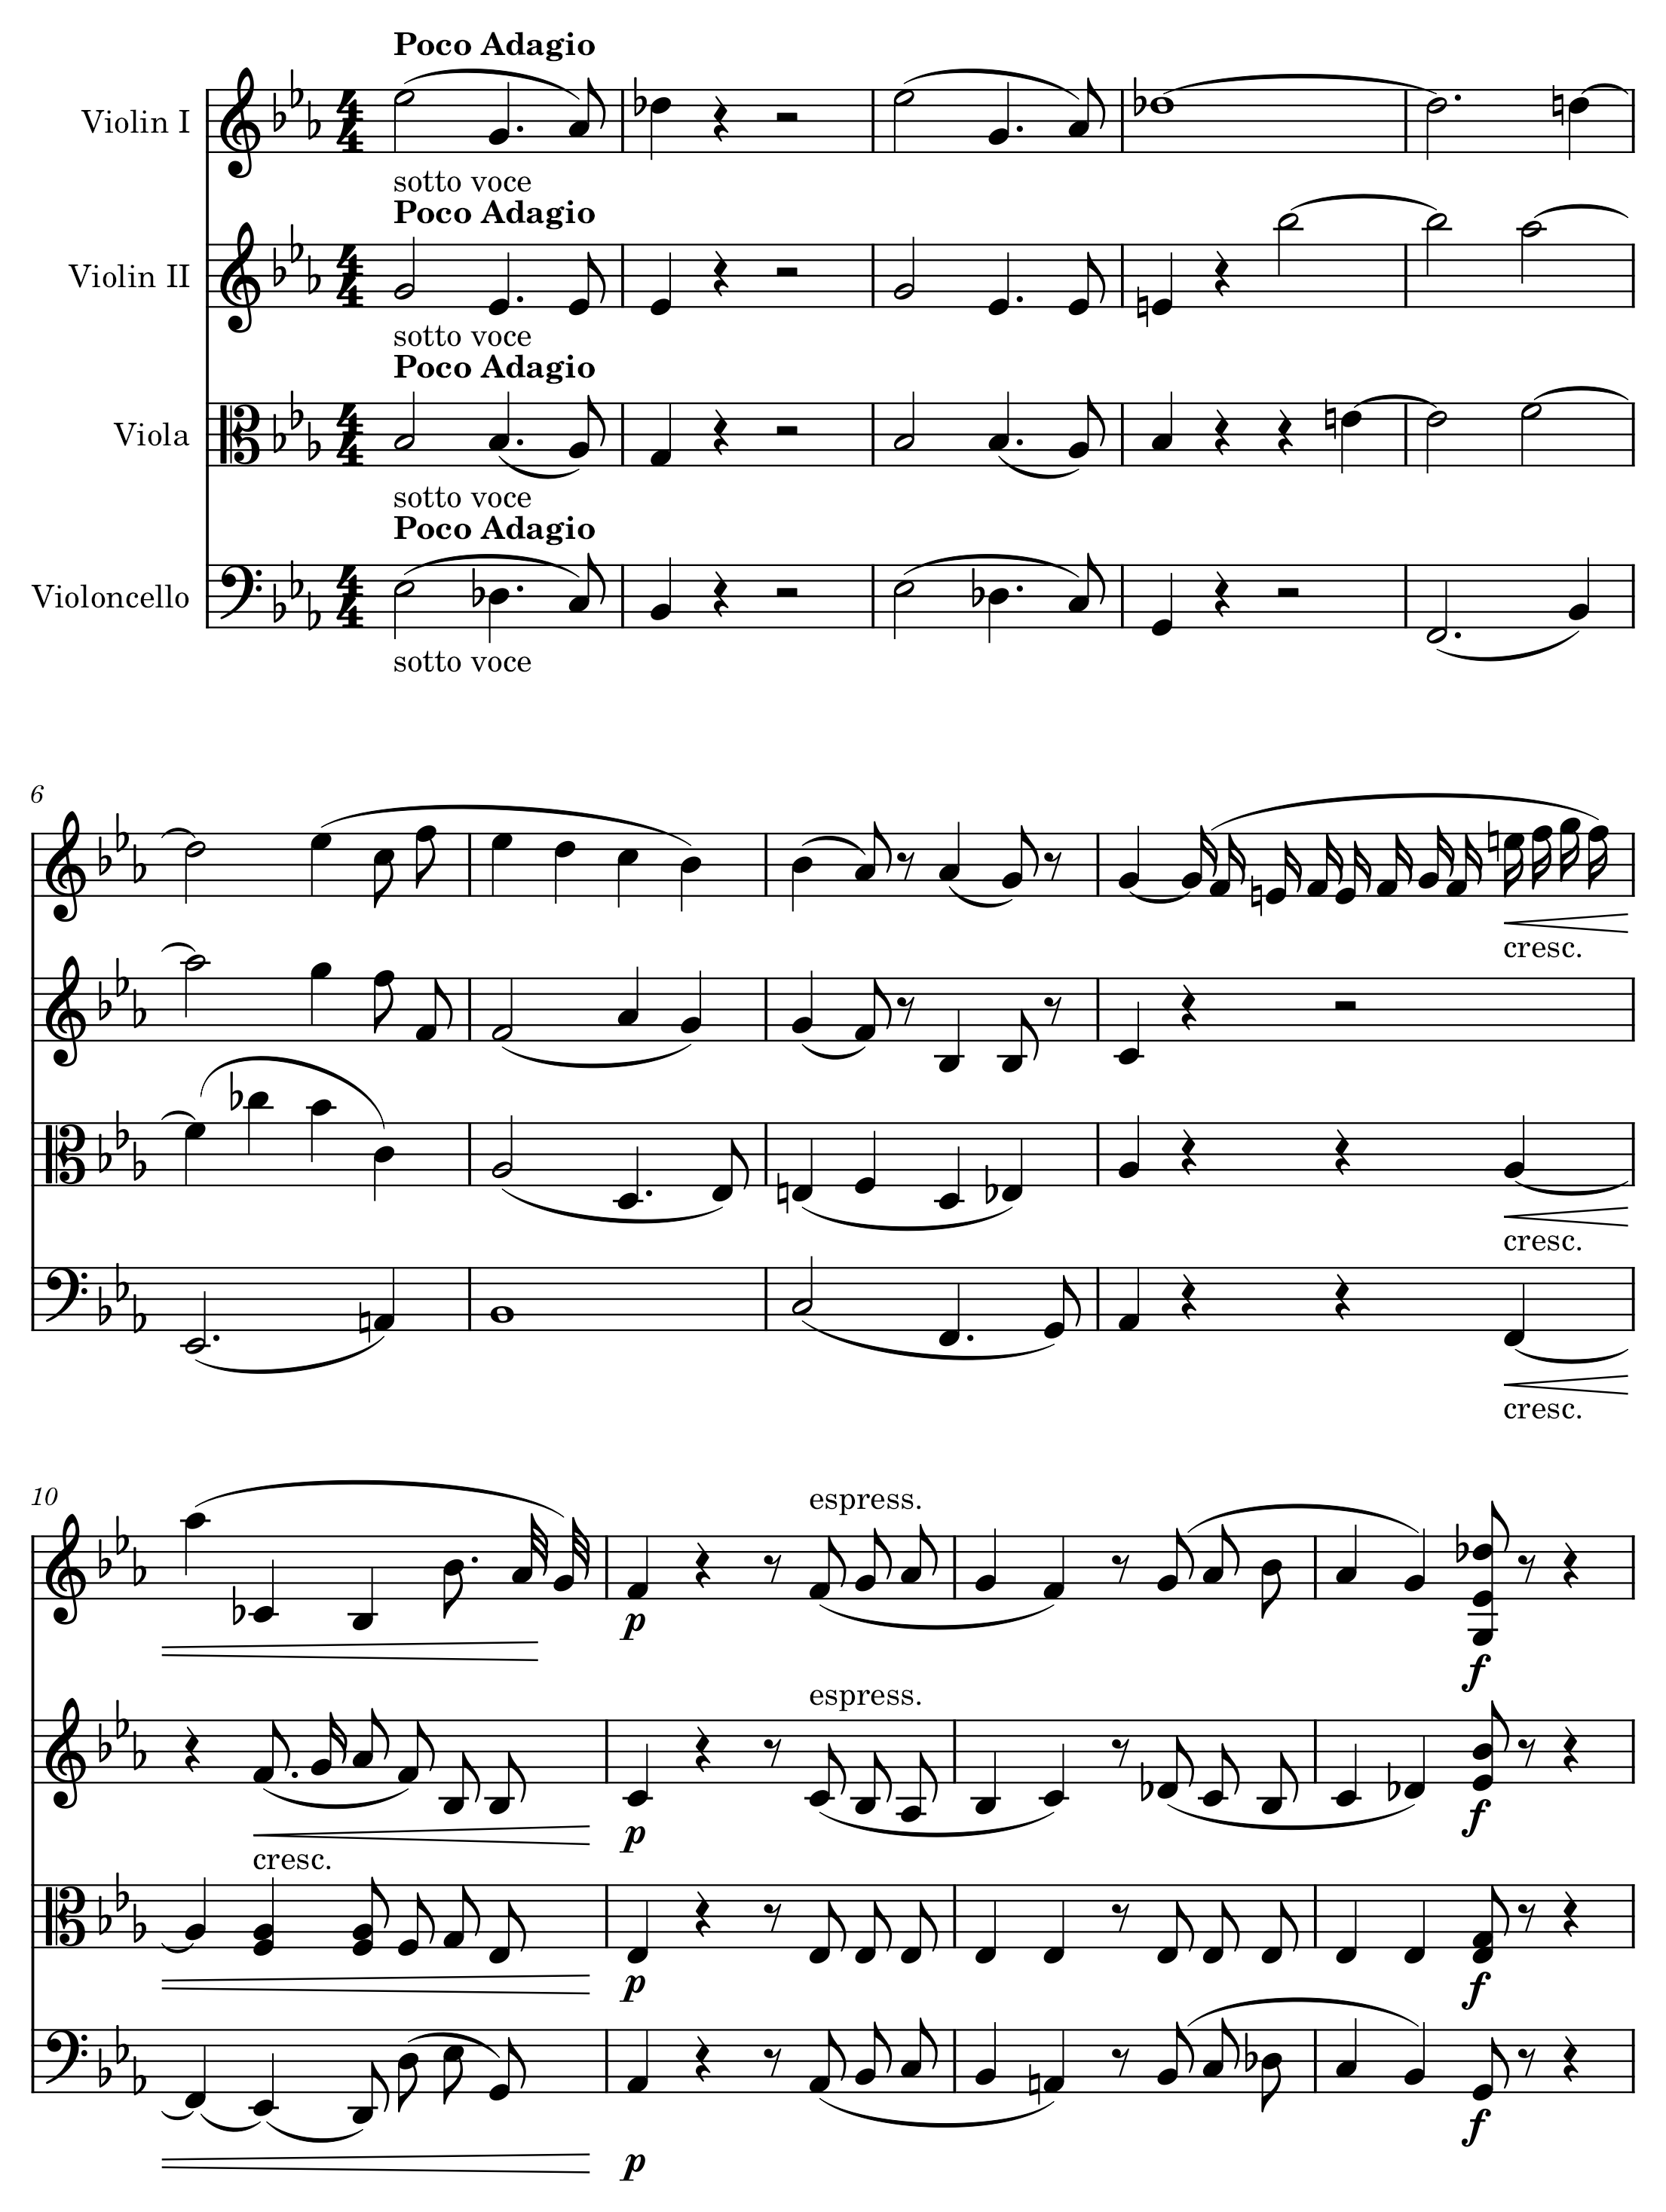
\includegraphics[width=0.5\textwidth]{../Figures/excerpt-1.png}
        \caption{String Quartet No.\ 10 by Ludwig van Beethoven}
    \end{figure}
\end{frame}

\begin{frame}{Phrase detection}
    Local boundary detection model (LBDM)
    \begin{figure}
        \centering
        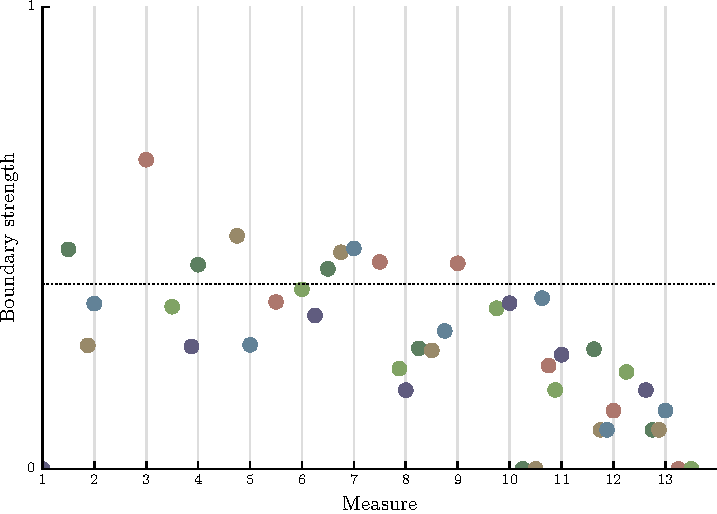
\includegraphics[width=0.75\textwidth]{../Figures/boundary_offset.pdf}
        \caption{Boundary strengths for the Violin I part}
    \end{figure}
\end{frame}

\begin{frame}{Problem graph}
    \begin{figure}
        \centering
        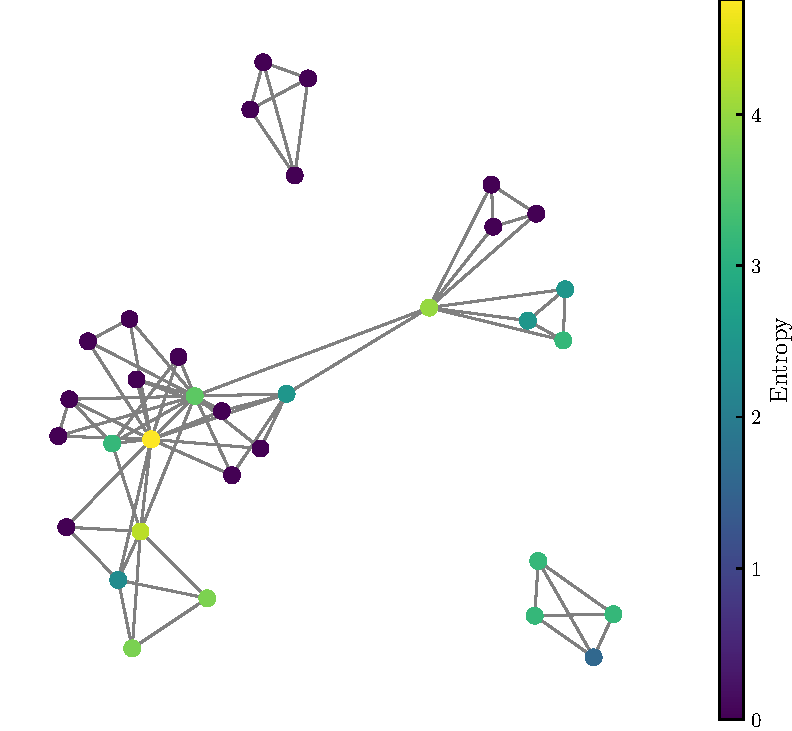
\includegraphics[width=0.75\textwidth]{../Figures/problemGraph.pdf}
    \end{figure}
\end{frame}

\begin{frame}{Solutions}
    \note{Lowest energy solution was -26.8 with a degeneracy of 34}
    \begin{figure}
        \centering
        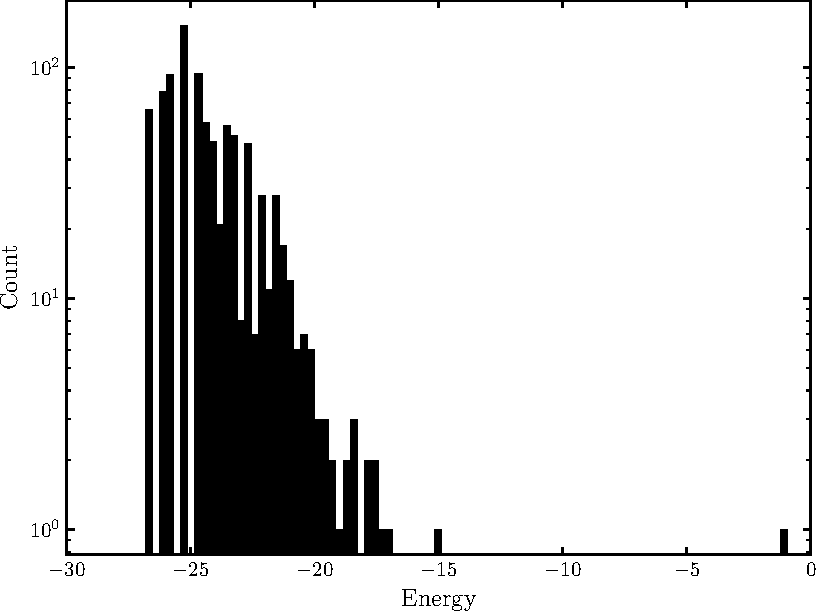
\includegraphics[width=0.9\textwidth]{../Figures/histogram.pdf}
        \caption{Solutions returned by the QPU}
    \end{figure}
\end{frame}

\begin{frame}{Example solution}

\end{frame}

\begin{frame}{Blocks}
    \begin{equation*}
        \oiint_A E\cdot dA=\frac{Q}{\varepsilon_0}
    \end{equation*}
    \pause
    \begin{block}{} % Empty title
        \centering
        The \emph{net electric flux} through any \alert{closed} surface is proportional to the \textbf{enclosed charge}.
    \end{block}

    \begin{alertblock}{Alert}
        This is an alert.
    \end{alertblock}

    \begin{exampleblock}{Example}
        This is an example.
    \end{exampleblock}
        
\end{frame}

\begin{frame}{Apperance sync}
    \begin{columns}

        \begin{column}{0.6\textwidth}
            \begin{itemize}
                \item<2-> Volume rate of flow equal to divergence
                \item<3-> Summed over entire volume
                \item<4-> Equal to net flow across the boundary
            \end{itemize}
        \end{column}

        \begin{column}{0.4\textwidth}
            \begin{figure}
                \centering
                    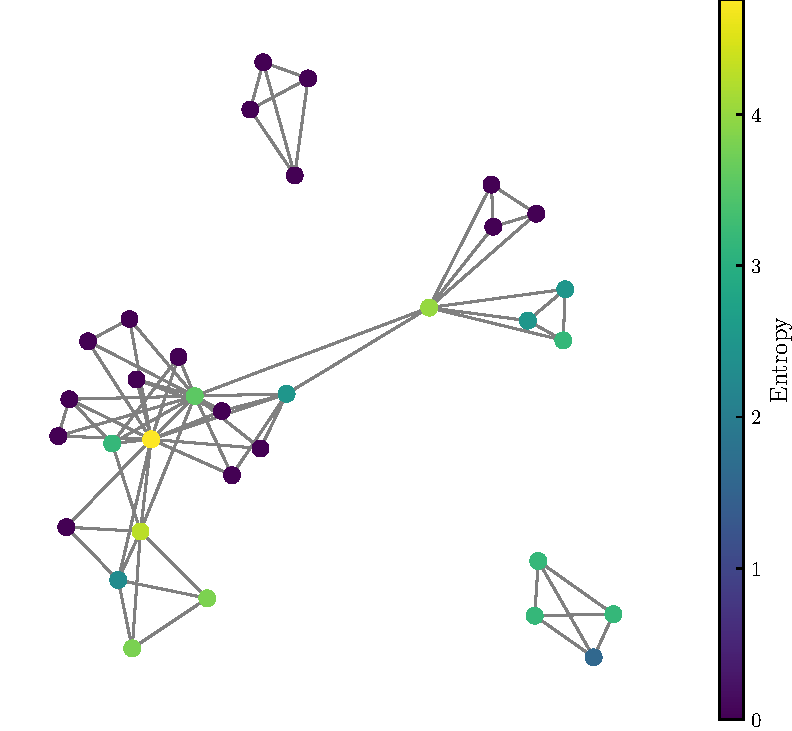
\includegraphics[width=\textwidth]{../Figures/problemGraph.pdf}
                    \caption{Source: Wikimedia Commons}
            \end{figure}
            \begin{equation*}
                % Syncing equation appearance with bullet points
                \onslide<3->{\iiint_V}\onslide<2->{\nabla\cdot\textbf{F}}\onslide<3->{\,dV}\onslide<4->{=\oiint_A \textbf{F}\cdot d\textbf{A}}
            \end{equation*}
        \end{column}

    \end{columns}
\end{frame}

\section{Conclusions}

\begin{frame}{Equation gather}
    \begin{gather*} % Multiple equations if alignment not important
        \nabla\cdot \textbf{E}=\frac{\rho}{\varepsilon_0} \\
        \nabla\cdot \textbf{B}=0 \\
        \nabla\times \textbf{E}=-\frac{\partial \textbf{B}}{\partial t} \\
        \nabla\times \textbf{B}=\frac1{c^2}\frac{\partial \textbf{E}}{\partial t}+\mu_0I
    \end{gather*}
\end{frame}

\end{document}